\documentclass[conference]{IEEEtran}
\IEEEoverridecommandlockouts
\usepackage{cite}
\usepackage{amsmath,amssymb}
\usepackage{booktabs}
\usepackage{graphicx}
\usepackage{xcolor}
\usepackage{url}
\usepackage[hidelinks]{hyperref}
\usepackage{tikz}
\usetikzlibrary{arrows.meta, positioning}
\newcommand{\code}[1]{\texttt{#1}}
\begin{document}
\title{Verifier Evaluation via Revision-Informed Trust, Abstention, and Suppression}
\author{%
\IEEEauthorblockN{S.V.Divya}
\IEEEauthorblockA{Department of CSE,\\ K.P.R College of Engineering\\ and Technology,\\ Coimbatore-642109.\\ divyasvvsb@gmail.com}
\and
\IEEEauthorblockN{R Harshan}
\IEEEauthorblockA{Department of CSE,\\ K.P.R College of Engineering\\ and Technology,\\ Coimbatore-642109.\\ harshanr695@gmail.com}
\and
\IEEEauthorblockN{P.M Akhil Jeikar}
\IEEEauthorblockA{Department of CSE,\\ K.P.R College of Engineering\\ and Technology,\\ Coimbatore-642109.\\ akhiljeikar06@gmail.com}
\and
\IEEEauthorblockN{T Ezhilperungo}
\IEEEauthorblockA{Department of CSE,\\ K.P.R College of Engineering\\ and Technology,\\ Coimbatore-642109.\\ ezhilperungotamizhazhagan@gmail.com}
\and
\IEEEauthorblockN{M Gurunathan}
\IEEEauthorblockA{Department of CSE,\\ K.P.R College of Engineering\\ and Technology,\\ Coimbatore-642109.\\ gurunathanmofficial@gmail.com}
}
\maketitle

\begin{abstract}
Large language models (LLMs) are increasingly used as verifiers of security findings: a static analyzer proposes a candidate, and a model adjudicates whether it is real. Whether such a verdict can be trusted is rarely measured. We apply the four-way decomposition, originally used to show that static analyzers flag constructs rather than vulnerabilities, to LLM verifiers, and add evidence gating, adversarial comments, composition, and calibration. On a 151-pair JavaVFC stratum, an evidence-gated verifier tracks the fix in 17.6\% of cases (95\% CI [16.7, 18.5], k=5), versus 0.7\% for the pattern matcher, while abstaining on 51.5\% of judgements and missing 79.1\% of fixes: its bottleneck is coverage, not accuracy. Adversarial comments evade 26\% (templates) to 50\% (adaptive), and nearly every evasion is an abstention rather than a false positive. Composing with a weaker verifier relocates trust rather than adding it. Blinding the commit message reduces detection by 18.1 points, exposing label leakage. We release a reproducible harness and argue that abstention and coverage should be reported as first-class outcomes.
\end{abstract}

\begin{IEEEkeywords}
abstention, adversarial robustness, calibration, code property graphs, evidence gating, large language models, program analysis, selective prediction, static analysis, vulnerability verification.
\end{IEEEkeywords}

\section{Introduction}

The process of automating vulnerability analysis adheres to a classic model: a policy is exploring an analysis tool and generates findings; and thus, to date, the process is employing LLM agents who analyse stores, apply analysis tools, and devise patches. And in every situation, the model checks whether the proposal received from the scanner is valid, yet now that the agents have entirely continued, can we rest on their competence, and isn't as easy as it may seem. The model can be precise in assessing the code, and yet wrong for the vulnerability itself, such as to take one instance, it can see that a potentially lethal code fragment is dangerous but not change it in the suggested patch; accept the fact that a particular value coming from the set of benchmarks is vulnerable without understanding the reasons behind it; come to a conclusion based on indication that's outside the training distribution. In our followed research paper, we prove that in case of static analysis, we can -ly differ between the ratio of commits when the candidate verdict changes with fixes and the benchmark true positive rate.

There are very real effects. Static analyzers have been plagued forever [6] by false positives. As well, they plague machine learning vulnerability detectors just as much [7], [8]. In the situation where the detector sits in front of remediation, there can be two ways that it goes wrong: it might corroborate something that isn’t a vulnerability (misapplication of effort, lowered trust). Only the same, even more worryingly, it might hide a real vulnerability. Prior research suggests that large language model security detectors are trivially worked by adversarial comments [9] and indirect prompting [10]; prior research has never looked into the whether an LLM detection actually follows through on a vulnerability, how that failure arises. But how it interacts with an opponent.

\noindent\textbf{Contributions.}

An instrument, like The four-way decomposition technique, explored earlier in the same paper in relation to static analyzers [5], is employed here for the first time in conjunction with LLM verifiers; this procedure makes possible us to support our claims with machine-verifiable proof; tell apart between false positives and abstentions in investigation; and report the coverage of the suggested method. The use, corpora and analyzers are publicly available.

A coverage-bounded finding, namely The evidence-based verifier is shown to report a fix with a rate of 17.6\% (95\% CI [16.7, 18.5], k=5) when compared to 0.7\% for the pattern matcher (representing 10-times over-reporting) and 0\% for CodeQL; in fact, according to the McNemar test (p$<$10−7), this result is noticeable. And yet, about 51.5\% of the time is being abstained by the evidence-based verifier and stops working to detect 79.1\% of the fixes; that's why, the primary issue isn't lack of sensitivity, but rather of silence.

Abstention defined as the attack surface. Any evasion can be hit thanks to abstention instead of making false positives in case of attacks; indeed, nobody can trick a classifier with comment-stripping mitigation.

Quantifiable leakage. After blanking the commit message, the detection reduces from 31.4 to 13.3\% (-18.1 percentage points): the commit message includes true labeling information, and the code itself is around 19 times more powerful compared to this tool.

Composition changing trust surface. the introduction of weak classifiers as a second filtering step is decreasing the recall without making any enhancement; indeed, evidence filtering doesn't rack up any recall cost (3:4, p=1.0).

A mistake finding in incorrect reading on the prescribed ground truth. What's more, the use of the scanning hint doesn't increase the number of held back cases. The analyzer has a recall of 0.905 and a precision of 0.734 when employing the OWASP Benchmark dataset including 2,740 labeled instances; still, the CIS doesn't refine the precision of the assessment as no model, either local 7B or cloud, rejects any false positive. Particular coverage is being needed by the verification process.

Precision and cost are, taken into the account. When n = 151, the cost of assessing roughly by eight times is being lessened by the disabling of the thinking; the verifier has good exactness (0.9\% constant-side false positives), but lacks stable calibration (ECE 0.116; [0.106, 0.131].

The paper mainly explores the extent of the proof, and so we consider it a advancement to measuring would-be effects rather than claiming them.

\section{Background and Related Work}

\subsection{LLM agents for vulnerability analysis}

LLM-assisted vulnerability discovery systems have been quickly evolving to include static analysis and symbolic execution with LLMs [4], and agentic frameworks such as VulAgentRL, Antares and EAVA include the examination into the pipeline [1], [3]; in fact, enhancements in discovery efficiency are being claimed by them, and don't measure if the verdict is in sync with the vulnerability, and usually don't show the coverage, precision trade-off of the verifier itself. Our metric is, as a practical matter, emphasizing on measuring the verdict accuracy rather than discovery efficiency.

\subsection{Verifiers and verifiable rewards}

VulAgentRL uses a property graph of code as both a tool and a verifier of rewards by node-level exact match [1]; Antares trains small models using verifiable rewards [2]; EAVA entails a combination of supervised fine-tuning and reinforcement learning while demanding indication for a verdict [3]. By “verifiable”, we mean the verifiability of the training signal, not the truthfulness of the inference-time verdict of the model, and don’t train; we ask.

\subsection{Adversarial robustness of LLM code analysis}

Prior work shows that LLM security detectors are steerable by adversarial source comments [9], by indirect prompt injection [10], and by insecure code generation [12], [13]; code models can also be hardened and adversarially tested [11]. We attack the verifier rather than the detector, split evasion by outcome (false positive vs. abstention), and include an adaptive attacker.

\subsection{Abstention, selective prediction, and calibration}

The process of choosing the right category is suggesting that refusal is an obstacle to tackle [14], the roadblock of spotting out-of-the-box items has been called a close subject of the recognition problem [15]. In plain words recently, it has become known that the majority of neural networks are often miscalibrated [16], which is directing to the emergence of a new topic in the field of large language models dealing with abstention, as models only are understanding what they're aware of [17]; in this regard, there are proper studies checking this topic [18]. As well, this topic is assessed for security verification and conclude that abstention serves as an instrument of defence and as the central goal and the biggest hurdle faced by a verifier.

\section{Method}

The pipeline is showed in Figure 1. The candidates are handled by a pinned analyzer as a pair; the verifier is needing to ground for the verdict from resolvable evidence; both the vulnerable and the repaired verdicts are then broken down and recapped. Comments may be introduced before verification by a rival.

\subsection{The four-way decomposition}

\begin{figure}[t]
\centering
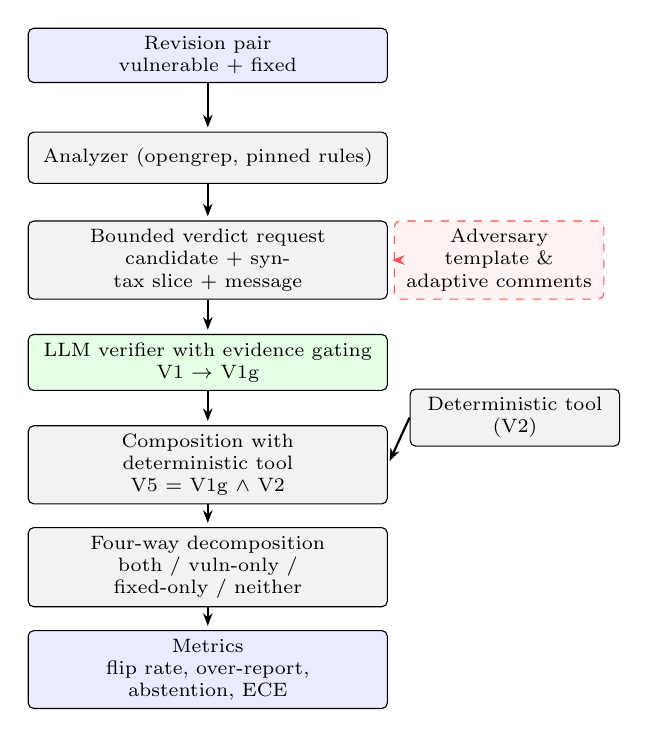
\begin{tikzpicture}[
  font=\scriptsize,
  >=Latex,
  box/.style={draw, rounded corners=2pt, align=center, inner sep=3pt,
              text width=4.35cm, minimum height=6.5mm},
  sidebox/.style={draw, rounded corners=2pt, align=center, inner sep=3pt,
                  text width=2.45cm, minimum height=6.5mm},
  io/.style={box, fill=blue!8},
  proc/.style={box, fill=black!5},
  ver/.style={box, fill=green!10},
  advbox/.style={sidebox, dashed, draw=red!70, fill=red!5},
  ar/.style={-{Stealth[length=1.6mm,width=1.2mm]}, thick, shorten >=1.5pt},
  dar/.style={-{Stealth[length=1.6mm,width=1.2mm]}, thick, dashed, red!70, shorten >=1.5pt}
]
\node[io]   (rev)   at (0,0)     {Revision pair\\ vulnerable $+$ fixed};
\node[proc] (an)    at (0,-1.3)  {Analyzer (opengrep, pinned rules)};
\node[proc] (req)   at (0,-2.6)  {Bounded verdict request\\ candidate $+$ syntax slice $+$ message};
\node[ver]  (judge) at (0,-3.9)  {LLM verifier with evidence gating\\ V1 $\rightarrow$ V1g};
\node[proc] (comp)  at (0,-5.2)  {Composition with deterministic tool\\ V5 $=$ V1g $\wedge$ V2};
\node[proc] (dec)   at (0,-6.5)  {Four-way decomposition\\ both / vuln-only / fixed-only / neither};
\node[io]   (met)   at (0,-7.8)  {Metrics\\ flip rate, over-report, abstention, ECE};

\node[advbox] (adv)  at (3.7,-2.6)  {Adversary\\ template \& adaptive comments};
\node[sidebox, fill=black!5] (tool) at (3.9,-4.6) {Deterministic tool\\ (V2)};

\draw[ar]  (rev)--(an);
\draw[ar]  (an)--(req);
\draw[ar]  (req)--(judge);
\draw[ar]  (judge)--(comp);
\draw[ar]  (comp)--(dec);
\draw[ar]  (dec)--(met);
\draw[dar] (adv.west)--(req.east);
\draw[ar]  (tool.west)--(comp.east);
\end{tikzpicture}
\caption{RewardAudit architecture. A revision pair is scanned by a pinned analyzer;
each candidate is turned into a bounded verdict request over a tree-sitter syntax
graph and the commit message. The verifier must ground its verdict in
resolvable evidence (V1$\rightarrow$V1g). An adversary (dashed) can inject comments
before verification, and a deterministic tool can be composed with the verifier.
Verdicts on the two revisions feed the four-way decomposition, which yields the
reported metrics.}
\label{fig:arch}
\end{figure}

We sort a verifier's decision to either one of four cells (Fig. 2) in case of a vulnerable/patched revision pair; and thus, vuln-only alone serves as an indicator of detection. Both suggests a verifier has reported a build that was there before fixing and after fixing the program, so the verdict couldn't have been made on basis of vulnerability; from these four categories, we compute the flip rate (vuln-only proportion), the naive coverage (proportion reporting a vulnerable revision) and their ratio, the over-reporting ratio, "Over reports 6×" hinting six finds in vulnerable version to one monitoring the fix.

\begin{figure}[t]
\centering
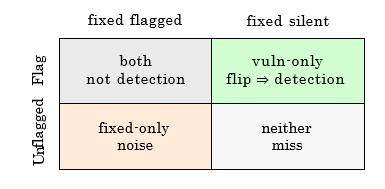
\includegraphics[width=\columnwidth]{humanized_figs/img02.png}
\par\medskip
\caption{Four way decomposition of a revision pair. Vuln-only is detection only. Both hints that the verifier flagged a build which existed pre-fix and post-fix.}
\end{figure}

\subsection{Verifier arms}

Here are four arms that take same input; and thus, v1 (LLM, Ungated): the decision made by the model. V1g (LLM, Gated): for all citations, there must be a valid syntax node reference; otherwise likely, the positive decision is considered unknown; indeed, v5 (Hybrid): flagged only if both gated LLM and tool decisions match. V2 (Tool): the pinned analyzer decision.

\subsection{Bounded verdict request and proof gating}

Store is always hidden from the model. Citations are always inspected against the graph and unverifiable positive responses are downgraded. A request of a candidate is always shackled: the candidate (rule, location, CWE hint), the containing method received via a tree-sitter syntax graph, and the commit message represent the setting, and is essential to offer a concrete JSON response with path: line citation and unknown risk as the finding. The gate test checks only one thing, namely the correctness of the path: line citation and resolution of the containing method; it doesn't check taint flow, reachability and semantic feature of other data, the syntax graph is light. As well, it isn't a dataflow engine (see Section VI); in turn, there's a reason why we never provide a whole file to assess.

\subsection{Adversary}

Templates, including five possible approaches to writing a comment (authority, sanitizer, tool-output, test-passed, and reviewed) are placed just before the suspected sink [9], and as well, the process looped up to three rounds, which is why evasion is separated into two categories, namely false positives and abstention. Adaptive - an attacker is modeled where a comment is written, the verdict by the verifier is gathered.

\section{Experimental Setup}

Corpora. (i) JavaVFC [20] (784 revision history; 327 usable single-file projects; and 324 materialised offline) consists of 151 revision pair that's subjected to fining down to a security level; the term security in the commit messages is combined with another random method (the screenshot version is in the manifest); this has been done after rolling-100 census and 51 extra pairs. In the whole stratum, all the values are, more accurately, subjected to 151 pairs of data, unless stated otherwise. A picked portion of robust security of 21 strong pairs has been chosen from related literature [5] for verification. (ii) There are 5 manually filtered pairs of vulnerable/fixed pairs in Python and 3 spyware in the canaries.(iii)21\_examples of Java have been identified in the related works [5]; there are issues regarding security entailing 18 unsafe revisions and 3 secure revisions; each file refers to one revision at one time and employs security methods in the commit message.

The tools employed were opengrep version 1.30.0, which included the previously tested 690-rule set of Java rules (hash: 77df32e0…) and a small ruleset with just 5 commands for Python. Even as, generating a global CodeQL database is impractical for this group of files, since javac fails after every 300 files, the findings were validated by running the previous test with one of the pairs, already shown to be fitting for the case. The current version of CodeQL (2.27.0) with the java-security-extended rules was used in a comparable fashion as the previous study, two versions in two CodeQL databases without a build for each rule.

Models. The 151 pair stratum runs are ran with mimo-v2.6-flash (k=5, cache disabled); legacy 21 pair sub-stratum is did with both mimo-v2.6-flash and deepseek-flash (k=5); all other families are benchmarked based on 5-pair Python tests. Five families against OpenAI's API compatibility, namely gpt-oss-120b, gpt-oss-20b, dwaen3.8-27b, deepseek-flash, and deepseek-v4-pro were tested.

Metrics \& Statistics. Each in turn model we introduce mean findings over 5 runs with 95\% bootstrap confidence interval; in fact, as, reasoning models are stochastic even at temperature of 0, the gathered span is also offered along with the confidence interval. Pairwise majority verdicts are checked against exact Mcnemar test on 151 pairs. Overreport appointed as

Reproducibility. Control reproduction and running of the test itself can (in practice) be ran completely offline; all assets protected by hash (pinning file).

\section{Results}

\subsection{Verifier dependence}

We start by asking whether the verdict follows the code or the model behind it; indeed, Table I answers on five Python pairs. gpt-oss-120b is reversing itself on four pairs and flags canary code once in three tries. gpt-oss-20b, qwen3.8-27b and deepseek-flash reverse on all five, and gpt-oss-20b also raises a canary false positive; prompt, setting and canaries are same in every run, so the difference belongs to the verifier. deepseek-v4-pro reverses on four and never disagrees with itself.

The chart is giving Table I a shape; three families sit at 100\% and two at 80\%; that spread isn't a difference in skill but in the willingness to change a verdict once the fix is generally employed. The column also is hiding the canary results, which is the point, including the two families that flag canary code, both gpt-oss versions, look ordinary here; a family is admitted or rejected on the canaries, which is mainly why the rest of the section reports arms rather than one score.

\subsection{LLM versus pattern matcher and CodeQL, and composition}

Neither deterministic baseline tracks fixes. On the 151 pairs the pattern matcher flips once (0.7\%) and nine further pairs flip under the both revisions, giving a tenfold over-reporting ratio; CodeQL flips on none. The gated verifier flips on 17.6\% of pairs (95\% CI [16.7, 18.5] over five runs), roughly twenty-five times the pattern matcher, and reports at 1.02×.

Over-report = (both + vuln\_only)/vuln\_only.

\begin{table}[t]
\centering
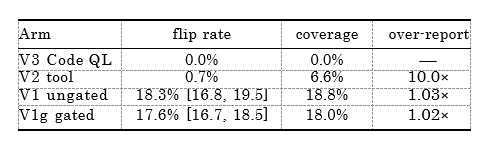
\includegraphics[width=\columnwidth]{humanized_figs/img05.png}
\caption{Verifier arms on the 151-pair security stratum (mimo-v2.6-flash, mean over k=5, 95\% CI; deterministic arms are a single run).}
\end{table}

Gating comes close to a true null - McNemar is giving 3:4 at p = 1.0; what's more, the false-positive rate falls from 0.8 to 0.6. Filtering unverifiable positives therefore costs almost nothing. Adding the tool as a second, weaker voice (V5) brings no proof and removes recall, because it can, in practice, only veto what the stronger verifier already accepted; indeed, composition goes the other way.

Over-reporting is telling a scanner that reports code from a verifier that reports a vulnerability; the pattern matcher is reaching 0.7\% only by flagging the same build before and after the fix ten times for every pair it genuinely is following. Both model arms sit near 1.0, and yet, nearly every positive they issue belongs to the revision where the defect was removed. What codeQL reports is nothing on the vulnerable side, which is leaving its ratio undefined rather than perfect.

CodeQL was the taint baseline. Over 151 pairs CodeQL flags no vulnerable revision; findings are appearing only in 22 fixed revisions; there's no deterministic taint result to compare on this data. The adapter is verified against a known case, java/sensitive-log (CWE-532) in commit efaa120ecc0d; a whole-directory, build-free database isn't workable for this corpus: javac exhausts memory and the export returns an empty SARIF, so each pair is analysed as two databases, as in our earlier study.

The price of gating is appearing here. What's more, on top of that, the two model arms miss 81.7\% and 82.4\%; in turn, the pattern matcher misses 99.3\% of the fixes, CodeQL misses all of them; in fact, measured on scored revisions, the gated arm is holding back on 51.5\% of requests and misses 79.1\% of fixes [77.2, 80.9]. A verifier that is, in practice, right about what it reports and silent on four fixes out of five is easy to trust and hard to use; indeed, anyone who is reading an abstention as a negative inherits the last bar.

\subsection{Adversarial comments}

Two attacks were tried, such as five fixed templates, and an adaptive attacker that's reading the verdict and retries up to three times. The authority template, which is claiming the input is checked upstream, worked best. By rate the adaptive attacker did better, avoiding 50\% of the time against 26\% for the template set. Almost every success was an abstention rather than a false positive, eight of nine for the templates and all three for the adaptive run.

deepseek-v4-pro vs. judge deepseek-flash. Stratum-scale attack and mitigation results are, explored above.

Stripping comments is the obvious defence, so we removed every comment with a tree-sitter pass before building the request and re-ran the subset.

Stripping made steering more typical, not less, namely 12.0\% with comments and 20.0\% without; and thus, every steered source in both arms ended in abstention, with no false positive; that fits the process, like the attacker needs uncertainty, not belief, so abstention is the surface being attacked. The rise isn't a real effect, since the two arms are holding diverse true positives (5 and 6), and the model isn't self-consistent at temperature zero; it does, though, rule the mitigation out.

\subsection{Detection effectiveness on a labelled benchmark}

We also ran the pipeline where ground truth exists, including the OWASP Benchmark for Java [19], 2,740 cases, 1,415 vulnerable and 1,325 safe; indeed, the pinned analyzer is strong there (recall 0.905, precision 0.734) and still raises false positives.

A matched sample of fifteen true and fifteen false positives was re-judged with and without the scanner's rule, message and CWE hint.

Two conclusions are following. Verification rejects almost no false positives - neither the local 7B nor the cloud model separates a close miss from a bug, so precision stays where the analyzer left it; blinding doesn't help either, namely without the hint, rejections don't rise, abstentions are growing and recall falls.

\begin{figure}[t]
\centering
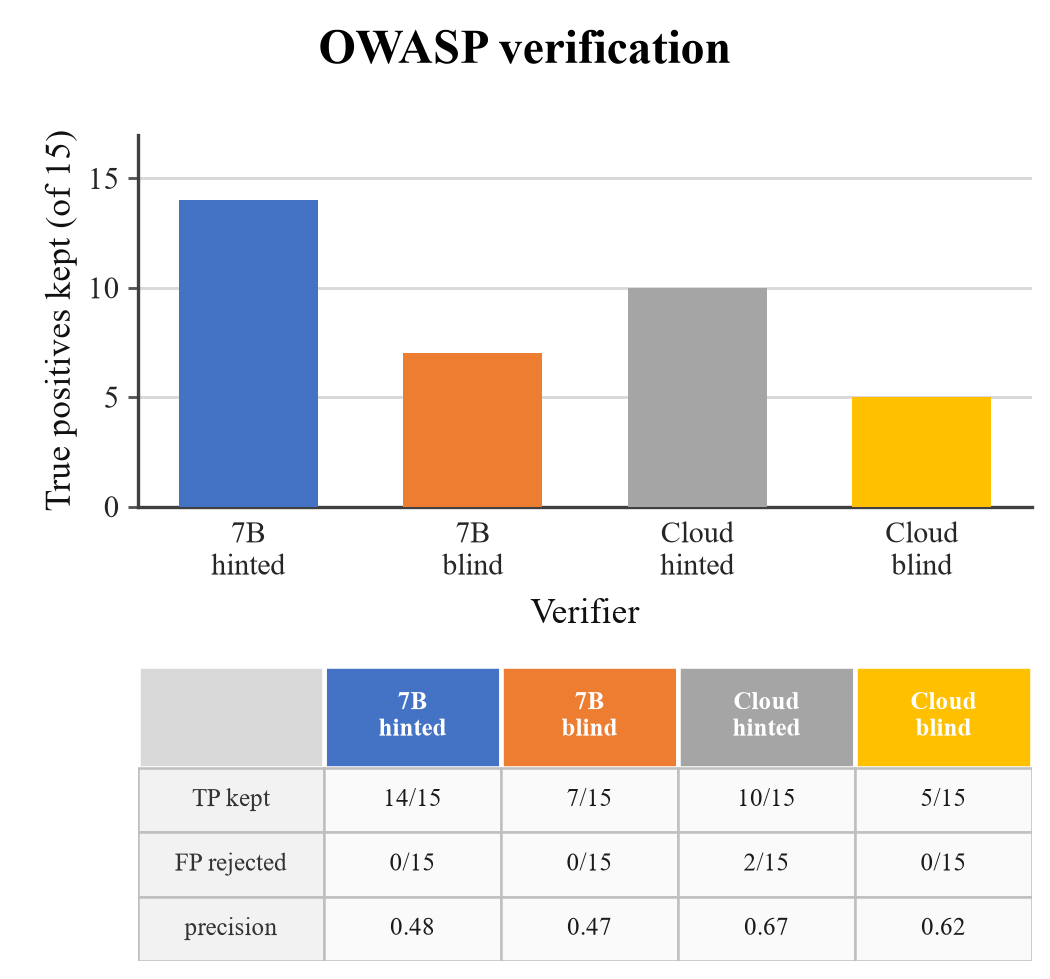
\includegraphics[width=\columnwidth]{humanized_figs/img15.png}
\par\medskip
\caption{Verification on the matched OWASP sample: true positives kept (bars) and the fate of the fifteen false positives (table); local and cloud verifiers, with and without the scanner hint.}
\end{figure}

The cloud verifier with the hint keeps 10 of 15 true positives and rejects 2 of 15 false positives, for precision 0.67; the local model is keeping 14 and rejects none, for 0.48; indeed, blinding hurts - dropping the rule, message and CWE hint halves kept true positives (14 to 7 locally, 10 to 5 in the cloud) and adds 14 and 9 abstentions out of 30. No arm is rejecting more than two of the fifteen, so none is separating a close miss from a bug; in fact, the hint is context the verifier needs, not a label it's repeating.

\section{Threats to Validity}

Scale. The scale of examination comprises 151 pairs of security problems in one corpus; in the cross-lingual experiment, five pairs of security problems were assessed, which made the cross-family investigation directional concerning the aim of the research. Labels. JavaVFC corpus served as the screening corpus: the previously ran audit revealed that only 18\% of the corpus really fixed. Input shape. Every revision is the individual record, which counts as the minimum of complexity for the methods employed to detect types of revisions and patterns. Evidence graph. Gating is using tree-sitter graph instead of sound dataflow engine, and, therefore, it can prove only the existence of the mentioned path/line and not the existence of the taint flow. Non-determinism. k=5 bootstrap ranges are showed. Reasoning models differ between runs at zero temperature; the average flip rate for five repeats for the legacy subset ranged from 28.6\% to 38.1\%.

\section{Conclusion and Future Work}

LLM security verifiers are much better than pattern matching and CodeQL, when it comes to tracking fixes. They're extremely well adjusted in their decisions about fixes, as embodied by just 0.9\% fixed-side false positives. But they aren't uniformly adjusted, and remain neutral to almost 50\% of their inputs. What's more, the obstacle isn't even relieved by the use of deterministic composition. Adversarial comments just worsen the situation. More often than not, the primary shortcoming of a security verifier is lying in coverage. As well, its adversarial target is abstention. Future research should encompass (i) running a census of 151 pairs with at least two extra model families, (ii) path-level security candidates testing on multi-file diffs, and (iii) concentrating on abstention and coverage of security agents.


\begin{thebibliography}{20}
\footnotesize
\setlength{\itemsep}{0pt}\setlength{\parsep}{0pt}
\bibitem{r1} Y. Li, T. Zhang, J. Liu et al., "Graph Is the Verifier: Agentic Reinforcement Learning for Interprocedural Vulnerability Detection," arXiv preprint arXiv:2607.26656, 2026.
\bibitem{r2} S. Vijay, A. Priyanshu, D. Chapoteau et al., "Antares: Foundation Models for Agentic Vulnerability Localization," arXiv preprint arXiv:2608.02407, 2026.
\bibitem{r3} S. Pan, Z. Zheng, J. Zhou et al., "Answer Is Cheap, Show Me the Evidence! Augmenting Automated Vulnerability Assessment with Evidence," arXiv preprint arXiv:2608.25905, 2026.
\bibitem{r4} N. Korda, G. Evron, "OpenAnt: LLM-Powered Vulnerability Discovery Through Code Decomposition, Adversarial Verification, and Dynamic Testing," arXiv preprint arXiv:2606.19149, 2026.
\bibitem{r5} RewardAudit Project, "A Benchmark Score That Nothing Can Be Concluded From: What the OWASP Benchmark Measures, and Why It Is Not Detection Capability," Technical report and artifact, 2026.
\bibitem{r6} C. Sadowski, E. Aftandilian, A. Eagle et al., "Lessons from Building Static Analysis Tools at Google," Communications of the ACM, 2018.
\bibitem{r7} S. Chakraborty, R. Krishna, Y. Ding et al., "Deep Learning Based Vulnerability Detection: Are We There Yet?," IEEE Transactions on Software Engineering, 2022.
\bibitem{r8} D. Arp, E. Quiring, F. Pendlebury et al., "Dos and Don'ts of Machine Learning in Computer Security," Proceedings of the 31st USENIX Security Symposium, 2022.
\bibitem{r9} Z. Wu, C. Nita-Rotaru, "ALIBI: Adaptive Agentic Attacks on LLM-Based Vulnerability Detectors via Adversarial Code Comments," arXiv preprint arXiv:2607.24964, 2026.
\bibitem{r10} K. Greshake, S. Abdelnabi, S. Mishra et al., "Not What You've Signed Up For: Compromising Real-World LLM-Integrated Applications with Indirect Prompt Injection," Proceedings of the 16th ACM Workshop on Artificial Intelligence and Security (AISec), 2023.
\bibitem{r11} J. He, M. Vechev, "Large Language Models for Code: Security Hardening and Adversarial Testing," Proceedings of the 2023 ACM SIGSAC Conference on Computer and Communications Security (CCS), 2023.
\bibitem{r12} H. Pearce, B. Ahmad, B. Tan et al., "Asleep at the Keyboard? Assessing the Security of GitHub Copilot's Code Contributions," 2022 IEEE Symposium on Security and Privacy (SP), 2022.
\bibitem{r13} N. Perry, M. Srivastava, D. Kumar et al., "Do Users Write More Insecure Code with AI Assistants?," Proceedings of the 2023 ACM SIGSAC Conference on Computer and Communications Security (CCS), 2023.
\bibitem{r14} Y. Geifman, R. El-Yaniv, "Selective Classification for Deep Neural Networks," Advances in Neural Information Processing Systems 30, 2017.
\bibitem{r15} D. Hendrycks, K. Gimpel, "A Baseline for Detecting Misclassified and Out-of-Distribution Examples in Neural Networks," International Conference on Learning Representations (ICLR), 2017.
\bibitem{r16} C. Guo, G. Pleiss, Y. Sun et al., "On Calibration of Modern Neural Networks," Proceedings of the 34th International Conference on Machine Learning (ICML), 2017.
\bibitem{r17} S. Kadavath, T. Conerly, A. Askell et al., "Language Models (Mostly) Know What They Know," arXiv preprint arXiv:2207.05221, 2022.
\bibitem{r18} L. Zheng, W. Chiang, Y. Sheng et al., "Judging LLM-as-a-Judge with MT-Bench and Chatbot Arena," Advances in Neural Information Processing Systems 36, 2023.
\bibitem{r19} OWASP Foundation, "OWASP Benchmark Project," 2026.
\bibitem{r20} JavaVFC authors, "JavaVFC: A Corpus of Vulnerability-Fixing Commits for Java," Zenodo dataset, 2026.
\end{thebibliography}
\end{document}
